\begin{frame}{Element System of equations}
\begin{columns}
\column{0.48\linewidth}
\begin{outline}
\1 Each element has
\2 Property matrix, $K_e$
\2 Unknown nodal values, $u_e$
\2 Some load, $L_e$
\1 Forms a linear system of equations
\1 Degrees of freedom per node varies by problem
\1 Element matrices are dense
\end{outline}

\column{0.48\linewidth}
\begin{center}
  \begin{align*}
    [K_e]\{u_e\} = \{L_e\}
  \end{align*}

  \vspace{1cm}

  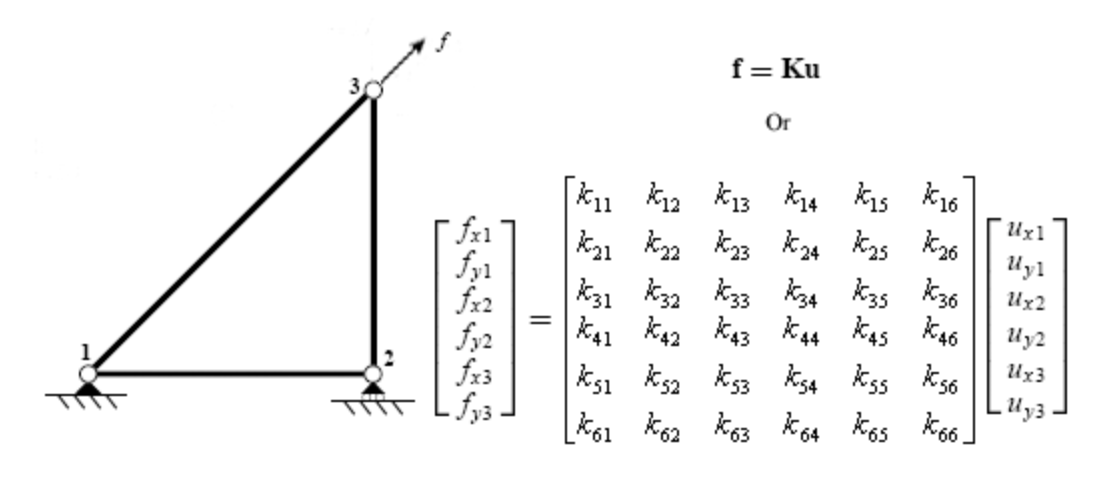
\includegraphics[width=5.5cm]{displacement_system.png}
\end{center}
\end{columns}
\blfootnote{From \href{https://fe4d.com/fe/intro/assets/DSMImage4.png}{fe4d}}
\end{frame}

\begin{frame}{Global Assembly and Solve}
  \begin{columns}
  \column{0.48\linewidth}
  \begin{center}
    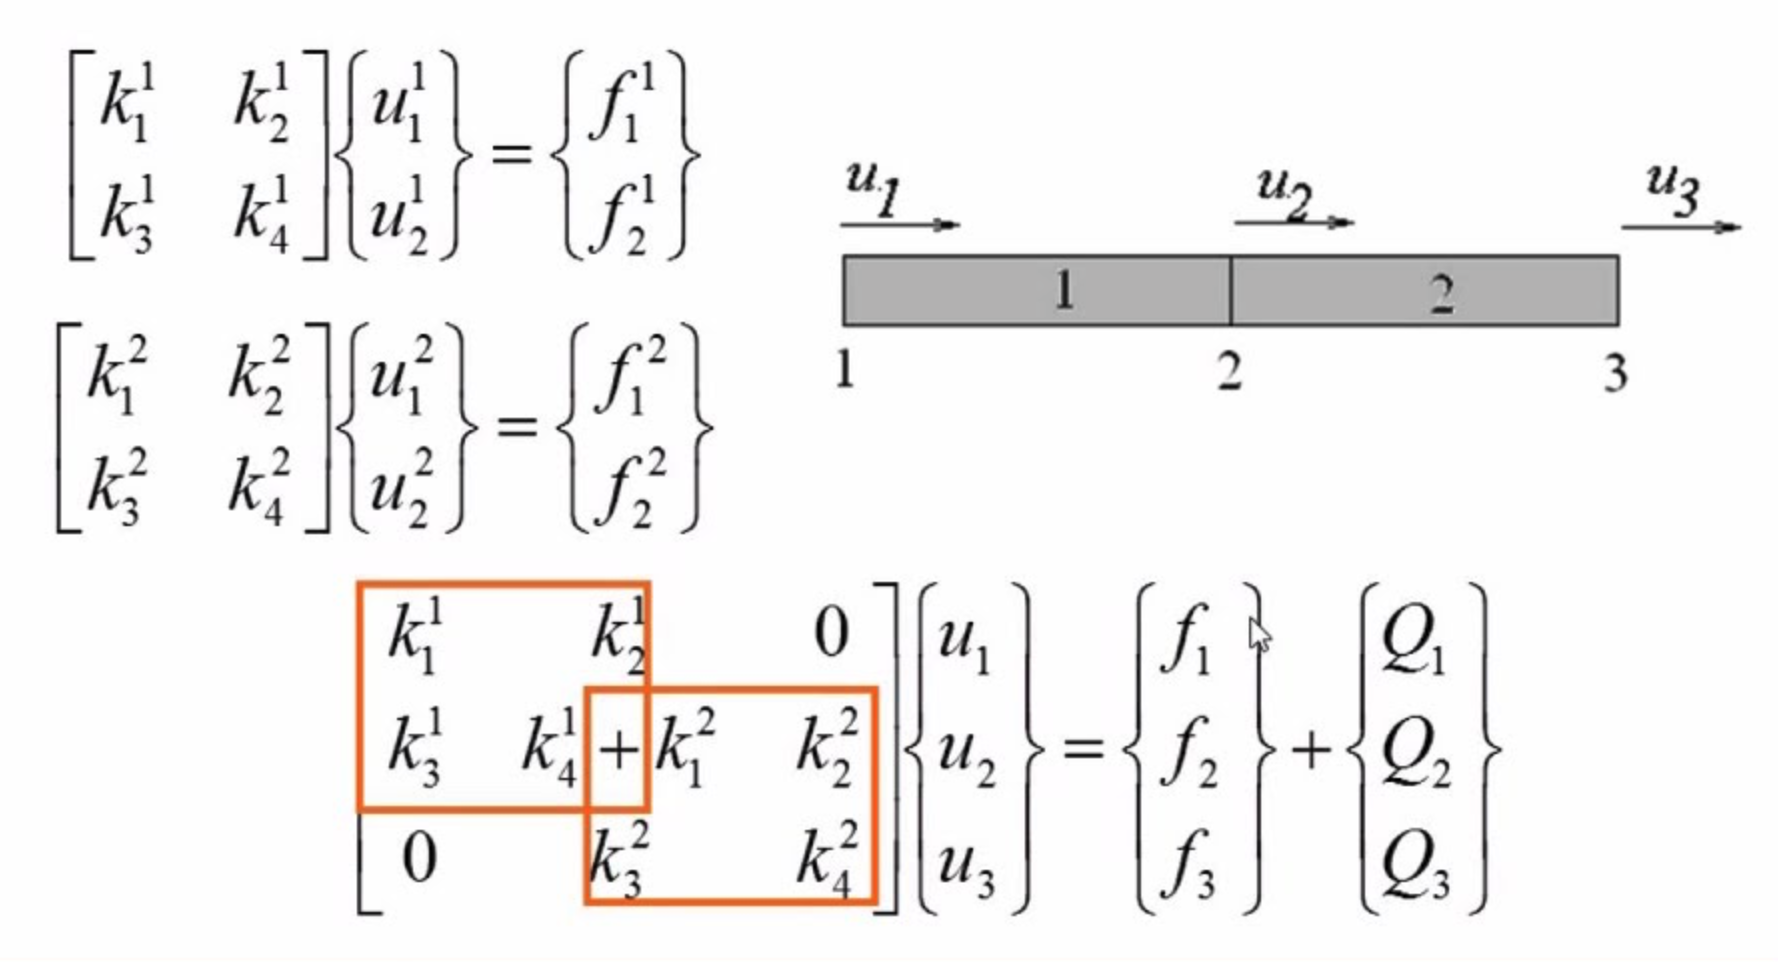
\includegraphics[width=5cm]{two_element_example.png}
  \end{center}

  \column{0.48\linewidth}
  \begin{center}
    \shadowimage[width=4cm]{sparsity_pattern.png}
  \end{center}
  \end{columns}
  \begin{center}
\begin{align*}
    [K]\{u\} = \{L\}
  \end{align*}
  \end{center}
  \blfootnote{From \href{https://www.youtube.com/watch?v=MoDPZoYtkDY}{FEM: Element Assembly}, \href{https://www.researchgate.net/profile/Ermanno-Affuso-2/publication/282929657/figure/fig1/AS:391480075145249@1470347531709/Sparsity-pattern-of-the-spatial-weight-matrix-W.png}{Research Gate}}
\end{frame}


